% =====================================================================
%  Group-Fair Stochastic Gradient Descent via Masked Optimal Transport
%  ICASSP submission -- 4 pages + 1 page references
%
%  Compile:  pdflatex main; pdflatex main
%
%  Markers you should sweep before submission:
%     %%FILLIN   -- a number or description only you can supply
%     %%CHECK    -- a claim worth re-reading against the code
%
%  Revision 2026-09-22: all \hr comments addressed. New figure
%  figs/motivation.pdf (Fig. 1) is produced by motivation.py; every
%  number quoted from it comes from that script.
% =====================================================================
\documentclass{article}
\usepackage{spconf,amsmath,amssymb,amsthm,graphicx,booktabs,multirow}
\usepackage{algorithm}
\usepackage{algpseudocode}
\algrenewcommand{\alglinenumber}[1]{\small #1:}
\usepackage[usenames,dvipsnames]{xcolor}
\usepackage{url}
\usepackage{balance}

% ---------------------------------------------------------------- macros
\newtheorem{theorem}{Theorem}
\newtheorem{lemma}[theorem]{Lemma}
\newtheorem{proposition}[theorem]{Proposition}
\newtheorem{corollary}[theorem]{Corollary}
\theoremstyle{definition}
\newtheorem{assumption}[theorem]{Assumption}
\newtheorem{remark}[theorem]{Remark}

\newcommand{\R}{\mathbb{R}}
\newcommand{\E}{\mathbb{E}}
\newcommand{\PP}{\mathbb{P}}
\newcommand{\Nn}[1]{[#1]}
\newcommand{\simplex}[1]{\Delta^{#1-1}}
\newcommand{\CVaR}{\mathrm{CVaR}}
\newcommand{\KL}{\mathrm{KL}}
\newcommand{\hr}[1]{\textcolor{blue}{#1}}
\newcommand{\Proj}{\Pi_{\mathcal{C}}}
\newcommand{\Reach}{\mathcal{P}(q,E)}
\newcommand{\avot}{\textsf{GAVOT}}
\newcommand{\avotcvar}{\textsf{GAVOT+CVaR}}
\DeclareMathOperator*{\argmin}{arg\,min}
\DeclareMathOperator*{\argmax}{arg\,max}
\newcommand{\best}[1]{\textbf{#1}}

% ---------------------------------------------------------------- title
\title{GROUP-FAIR STOCHASTIC GRADIENT DESCENT \\ VIA MASKED OPTIMAL TRANSPORT}

\name{Herlock (SeyedAbolfazl) Rahimi \quad Amtej Sodhi \quad Vihaan Goyal \quad Dionysis Kalogerias%
\thanks{\small This work is supported by NSF under Grant 2242215.
Amtej~Sodhi is a senior at Stuyvesant High School, New York, NY.
Vihaan~Goyal is a junior at Westhill High School, Stamford, CT.}}

\address{Department of Electrical and Computer Engineering, Yale University, New Haven, CT, USA\\
{\normalsize\texttt{\{herlock.rahimi, dionysis.kalogerias\}@yale.edu}}\\
{\normalsize\texttt{\{vihaan.goyal1512, amtejsodhi\}@gmail.com}}}

\begin{document}
\ninept
\maketitle
\pagestyle{empty}\thispagestyle{empty}

\begin{abstract}
Minibatch stochastic gradient descent (SGD) weights each group of a
population by how often it appears in a batch, not by the importance the
objective assigns to it, so under imbalance it minimizes a surrogate that
favors well-represented groups whatever the stepsize. We show that every
rule weighting the groups of a batch optimizes a weighting confined to a
polytope fixed by the sampler, which contains the target exactly when a
masked optimal transport problem between the batch-composition law and the
importance distribution is feasible. The resulting method, \avot{},
reweights each batch with a Sinkhorn plan computed once; its gradient is
unbiased for the target risk, and it converges at the $O(1/\sqrt{T})$ rate
of SGD with access to every group. When coverage fails, an alignment gap
computable before training predicts whether transport pays, and a
mean--conditional-value-at-risk (CVaR) layer certifies the target risk.
Experiments on Adult and IMDb-Wiki confirm the predictions.
\end{abstract}

\begin{keywords}
Group fairness, imbalanced learning, stochastic gradient descent, optimal
transport, conditional value at risk.
\end{keywords}

% =====================================================================
\section{Introduction}
\label{sec:intro}
% =====================================================================

Training data rarely represent a population evenly, and the
under-represented pay for it at deployment. Face-analysis systems err most
on the demographic intersections least present in their training data
\cite{buolamwini2018gender}, speech recognizers make markedly more errors
for Black than for white speakers \cite{koenecke2020speech}, and imbalanced
regression errs most where labels are scarce \cite{yang2021dir}; when
poorly served users disengage, later data contain even fewer of them
\cite{hashimoto2018repeated}. Imbalance is the norm
\cite{he2009imbalanced}, so a training method should be judged by the risk
it attains on every group.

Formally, let $\mathcal{X}\subseteq\R^{d_x}$ and $\mathcal{Y}$ be the input
and output spaces ($\mathcal{Y}=\R$ in regression, a finite label set in
classification) and $\Nn{N}$ a set of \emph{groups}, e.g.\ demographic
categories. Data are triples $(X,Y,G)\sim\PP$ on
$\mathcal{X}\times\mathcal{Y}\times\Nn{N}$; group $i$ has \emph{prevalence}
$\pi_i\triangleq\PP[G=i]$ and conditional law $\mathcal{D}_i$ of $(X,Y)$.
A predictor $m(\cdot\,;\theta):\mathcal{X}\to\hat{\mathcal{Y}}$,
$\theta\in\mathcal{C}\subseteq\R^{d}$, is scored by a loss
$\ell:\hat{\mathcal{Y}}\times\mathcal{Y}\to\R_+$, and group $i$ has
\emph{risk} $f_i(\theta)\triangleq\E_{\mathcal{D}_i}[\ell(m(X;\theta),Y)]$.
For $w\in\simplex{N}$ let $F_w\triangleq\sum_iw_if_i$,
$f\triangleq(f_1,\dots,f_N)$ and $\theta^\star_w\in\argmin_{\mathcal{C}}F_w$.
The population risk is $F_\pi$, but the learner declares an
\emph{importance distribution} $p\in\simplex{N}$ (uniform,
inverse-prevalence, or set by a fairness specification
\cite{mohri2019agnostic,li2020fair}), and the task is
\begin{equation}
\min_{\theta\in\mathcal{C}}\ F_p(\theta)=\textstyle\sum_{i=1}^{N}p_if_i(\theta).
\label{eq:target}
\end{equation}

Minibatch SGD solves \eqref{eq:target} in practice. At step $t$ a sampler
returns a \emph{minibatch} $B^t=\{(x^t_k,y^t_k,g^t_k)\}_{k=1}^{b}$, and
\emph{uniform} minibatch SGD, which draws the $b$ triples i.i.d.\ from
$\PP$, updates $\theta^t=\Proj(\theta^{t-1}-\eta_t\hat g^t_{\mathrm u})$
with stepsize $\eta_t$, Euclidean projection $\Proj$ onto $\mathcal{C}$,
and batch gradient
\begin{equation}
\begin{aligned}
\hat g^t_{\mathrm u}&\triangleq\tfrac1b\textstyle\sum_{k=1}^{b}\nabla_\theta\ell\big(m(x^t_k;\theta^{t-1}),y^t_k\big),\\
\E\big[\hat g^t_{\mathrm u}\mid\theta^{t-1}\big]&=\textstyle\sum_{i=1}^{N}\pi_i\nabla f_i(\theta^{t-1})=\nabla F_\pi(\theta^{t-1}),
\end{aligned}
\label{eq:introbias}
\end{equation}
where the mean follows because each summand is drawn from the mixture
$\sum_i\pi_i\mathcal{D}_i$.
Uniform SGD thus descends $F_\pi$ whatever $p$ is, and approaches
$\theta^\star_\pi$, not $\theta^\star_p$, for every horizon and stepsize
schedule.

Which groups pay follows from optimality alone. Adding
$F_w(\theta^\star_w)\le F_w(\theta^\star_{w'})$ and
$F_{w'}(\theta^\star_{w'})\le F_{w'}(\theta^\star_w)$ gives, without
convexity,
\begin{equation}
\big\langle w-w',\,f(\theta^\star_w)-f(\theta^\star_{w'})\big\rangle\le 0
\qquad\forall\,w,w'\in\simplex{N},
\label{eq:mono}
\end{equation}
so group risks move against the weights. For two groups with $\pi_2<p_2$
the same inequalities give $f_2(\theta^\star_\pi)\ge f_2(\theta^\star_p)$
and $f_1(\theta^\star_\pi)\le f_1(\theta^\star_p)$, and SGD serves the
majority at the minority's expense. Fig.~\ref{fig:motivation} shows this on
a two-group regression with prevalences $0.9$ and $0.1$. Uniform SGD leaves
the minority an MSE six times the majority's, while our method, on the same
batches, reaches $\theta^\star_p$ for the uniform target, cutting the
minority's MSE from $1.03$ to $0.16$ at the price of $0.17\to0.39$ on the
majority.

\begin{figure}[t]
\centering
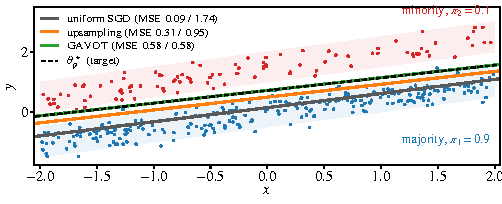
\includegraphics[width=\columnwidth]{figs/motivation.pdf}
\vspace{-16pt}
\caption{Two-group linear regression ($900/100$ samples in the shaded
ranges), i.i.d.\ batches of $b{=}8$, $5$ seeds; legend, group MSEs.
$p=(\frac12,\frac12)$ is reachable as $r_2=1-0.9^8\ge p_2$.}
\label{fig:motivation}
\vspace{-10pt}
\end{figure}

Existing remedies act on the sampler, the loss or the objective.
Resampling \cite{he2009imbalanced,chawla2002smote} and group-balanced
sampling \cite{idrissi2022simple} rebalance the batches; loss reweighting by
class \cite{cui2019classbalanced} or label \cite{yang2021dir} frequency and
margin or logit adjustment \cite{cao2019ldam,menon2021logit} favor rare
classes, although importance weights fade once a deep network separates the
data \cite{byrd2019importance}; importance sampling for SGD
\cite{needell2014sgd,katharopoulos2018not} reduces gradient variance without
changing the objective. Group distributionally robust optimization (DRO)
minimizes the worst group risk \cite{sagawa2020dro}, variants dispense with
group labels \cite{hashimoto2018repeated,liu2021jtt}, CVaR and DRO
objectives hedge over reweightings of the data
\cite{namkoong2017variance,levy2020large,curi2020adaptive}, and constrained
and reductions methods impose group-wise requirements
\cite{hardt2016equality,agarwal2018reductions,cotter2019twoplayer,chamon2020pacc,chamon2023nonconvex}.
These
methods change what is optimized; we ask a question one level lower. When
the learner does not choose which groups a batch contains, as in streaming,
sharded or access-restricted pipelines, its only lever is how the groups
present are weighted. \emph{Can these weights make SGD optimize the
declared $p$ exactly?}

Our remedy comes from our earlier work on a different problem, federated
learning, where a server aggregates updates from whichever clients
participate in a round; \textsf{FedAVOT} \cite{rahimi2025fedavot} and
\textsf{FedeRage} \cite{rahimi2026federage} correct the mismatch between
the participation law and the prescribed weights, \textsf{FedAVOT} by a
masked optimal transport (MOT) problem.
%%CHECK one-line description of FedeRage's role
Minibatch SGD has no clients or communication but the same combinatorics,
the groups present in a batch playing the participating clients.
Translating the construction, we make four contributions.
\begin{enumerate}\itemsep0pt\parskip0pt\topsep2pt
\item We prove that every normalized, label-dependent rule for weighting
the groups of a batch, uniform SGD included, is a stochastic subgradient
method on a surrogate risk whose weighting lies in a polytope fixed by the
batch-composition law, with a bias no number of iterations removes.
\item Inspired by MOT in federated learning, we devise \avot{}, which
reweights each batch by a Sinkhorn plan computed once. Under a Hall-type
coverage condition its gradient is unbiased for $\nabla F_p$ and
$\E F_p(\bar\theta_T)-\min F_p\le DG/\sqrt{T}$, the bound of SGD with
access to every group.
\item Beyond coverage, we split the excess risk into an alignment gap
computable before training and an optimization residual, and show that a
mean--CVaR layer bounds the target risk at rate $O(\kappa/\sqrt{T})$,
$\kappa=\gamma+(1-\gamma)/\alpha$.
\item Experiments on Adult and IMDb-Wiki support the analysis, with
transport lowering the target and rarest-group risks and its advantage
changing sign where predicted.
\end{enumerate}

% =====================================================================
\section{Problem Formulation}
\label{sec:setup}
% =====================================================================

The analysis covers any sampler. The \emph{active set}
$A^t\triangleq\{g^t_k\}_{k\le b}$ of groups present in $B^t$ takes values
in a family $\{A_j\}_{j\in\Nn{J}}$ of nonempty subsets of $\Nn{N}$, with
\emph{composition law} $q_j\triangleq\PP[A^t=A_j]$ and bipartite
\emph{mask} $E\triangleq\{(i,j):i\in A_j\}$. Group $i$ appears with
\emph{observation rate} $r_i\triangleq\PP[i\in A^t]=\sum_{j:\,i\in A_j}q_j$,
which is $1-(1-\pi_i)^b$ under i.i.d.\ sampling and $K/N$ when $K$ of the
$N$ groups are drawn uniformly, so a group whose prevalence is below the
resolution of the batch is absent from most batches. For $i\in A^t$ let
$g^t_i$ and $\hat f^t_i$ be the stochastic subgradient and the loss at
$\theta^{t-1}$, averaged over the examples of group $i$ in $B^t$.

\begin{assumption}
\label{ass:std}
$\mathcal{C}$ is convex and compact with diameter $D$; each $f_i$ is convex
and continuous on $\mathcal{C}$ with $0\le f_i\le M$; conditionally on
$\theta^{t-1}$ and on the labels of $B^t$, the examples of each $i\in A^t$
are i.i.d.\ from $\mathcal{D}_i$, so that
$\E[g^t_i\mid\theta^{t-1},A^t]\in\partial f_i(\theta^{t-1})$, and
$\E[\|g^t_i\|^2\mid\theta^{t-1},A^t]\le G^2$.
\end{assumption}

A \emph{group-weighting rule} replaces $\hat g^t_{\mathrm u}$ by
$\hat g^t=\sum_{i\in A^t}w^t_ig^t_i$, with $w^t\in\simplex{N}$ supported
on $A^t$ and depending on $B^t$ only through its labels. Uniform SGD is
$w^t_i=\widehat\pi^t_i$, the batch share of group $i$, and per-batch
upsampling $w^t_i\propto p_i/r_i$ is another. Averaging over the batch
given its composition and then over $A^t\sim q$ yields the objective of
every rule.

\begin{proposition}[Reachable objectives]
\label{prop:surrogate}
Under Assumption~\ref{ass:std}, a group-weighting rule is a stochastic
subgradient method on $F_{\tilde p}$, where
$\tilde p_i=\sum_{j:\,i\in A_j}q_j\,\E[w^t_i\mid A^t=A_j]$ lies in the
\emph{reachable set}
\begin{equation}
\Reach\triangleq\big\{\Gamma\mathbf 1_J:\ \Gamma\in\R_+^{N\times J},\
\mathbf 1_N^\top\Gamma=q^\top,\ \mathrm{supp}(\Gamma)\subseteq E\big\},
\label{eq:reach}
\end{equation}
so $\tilde p_i\le r_i$; uniform SGD under i.i.d.\ sampling has
$\tilde p=\pi$. Moreover $|F_p-F_{\tilde p}|\le M\|p-\tilde p\|_1$ on
$\mathcal{C}$, hence $F_p(\theta^\star_{\tilde p})-F_p(\theta^\star_p)\le
2M\|p-\tilde p\|_1$, a bias no number of iterations removes.
\end{proposition}
\noindent\emph{Proof sketch.} Given $A^t=A_j$, Assumption~\ref{ass:std}
yields $\E[\hat g^t\mid\theta^{t-1},A_j]=\sum_{i\in A_j}\E[w^t_i\mid
A_j]\,s_i$ with $s_i\in\partial f_i(\theta^{t-1})$, and
$\Gamma[i,j]\triangleq q_j\E[w^t_i\mid A^t=A_j]$ meets the constraints of
\eqref{eq:reach} because $w^t$ sums to one on $A_j$; the bounds follow from
$0\le f_i\le M$ (cf.\ \cite{rahimi2025agnostic}). \hfill$\square$

Hence $p$ shapes the iterates only through the weights and is optimized
exactly only if $p\in\Reach$. By \eqref{eq:mono}, the groups a rule
under-weights relative to $p$ are those whose risk rises, and no rule gives
a group more weight than its observation rate. It remains to find a rule
that reaches $p$ when this is possible, and the best one when it is not.

% =====================================================================
\section{Group-Fair SGD by Masked Optimal Transport}
\label{sec:gavot}
% =====================================================================

By Proposition~\ref{prop:surrogate}, a rule reaches $p$ exactly when it is
induced by a $\Gamma$, with $\Gamma[i,j]$ the mass composition $A_j$ sends
to group $i$, solving the \emph{masked optimal transport} problem
\begin{equation}
\Gamma\mathbf 1_J=p,\qquad \mathbf 1_N^\top\Gamma=q^\top,\qquad \Gamma\ge 0,
\qquad \mathrm{supp}(\Gamma)\subseteq E .
\label{eq:mot}
\end{equation}
Each solution induces the deterministic rule $w^t=W[\cdot,j(t)]$, where
$A^t=A_{j(t)}$ and $W\triangleq\Gamma\,\mathrm{diag}(q)^{-1}$ has columns
that are probability vectors on their compositions. Unlike classical
transport \cite{villani2009,peyre2019} there is no cost, the mask forbids
weighting absent groups, and existence is a supply--demand question on the
bipartite graph $E$, settled by flow duality
\cite{hall1935,fordfulkerson1956}.

\begin{theorem}[Coverage, one-sided form of {\cite[Thm.~1]{rahimi2025fedavot}}]
\label{thm:feas}
Problem \eqref{eq:mot} is feasible, i.e.\ $p\in\Reach$, if and only if
\begin{equation}
\textstyle\sum_{i\in I}p_i\;\le\;\sum_{j:\,A_j\cap I\neq\emptyset}q_j
\qquad\forall\,I\subseteq\Nn{N}.
\label{eq:hall}
\end{equation}
Taking $I=\{i\}$ and $I=\Nn{N}\setminus\{i\}$, feasibility requires
$\PP[A^t=\{i\}]\le p_i\le r_i$ for every $i$.
\end{theorem}
\noindent The singleton conditions are checked before training, and
the \emph{infeasible mass} $\nu\triangleq\sum_{i:\,p_i>r_i}p_i$, zero on
every feasible instance, measures how much of the target is out of reach.
Under i.i.d.\ sampling $p_i\le r_i$ means $b\ge\log(1-p_i)/\log(1-\pi_i)$,
under $K$-of-$N$ sampling $p_i\le K/N$.

When \eqref{eq:hall} holds, Sinkhorn scaling of the indicator of $E$ to the
marginals $(p,q)$ \cite{sinkhorn1967,cuturi2013,peyre2019} returns a
solution once, offline, at $O(|E|)$ per sweep, with $q$ given by the
sampler or estimated in one pass over the data. Algorithm~\ref{alg:gavot}
is the resulting method, \avot{}; $\gamma=1$ is the risk-neutral rule and
$\gamma<1$ the layer of Sec.~\ref{sec:cvar}.

\begin{algorithm}[t]
\caption{\avot{}: group-fair SGD by masked transport}
\label{alg:gavot}
\small
\begin{algorithmic}[1]
\Require $p$, $(q,\{A_j\},E)$, stepsizes $\eta_t$, horizon $T$,
$(\alpha,\gamma)\in(0,1]^2$
\State $\Gamma\leftarrow$ Sinkhorn scaling of $\mathbf 1_E$ to $(p,q)$;
$\ W\leftarrow\Gamma\,\mathrm{diag}(q)^{-1}$ \Comment{offline}
\State $\theta^0\in\mathcal{C}$, $\ \tau^0\in[0,M]$
\For{$t=1,\dots,T$}
  \State draw $B^t$; find $j$ with $A_j=A^t$; get $g^t_i,\hat f^t_i$, $i\in A^t$
  \State $c^t_i\leftarrow\mathbf{1}\{\hat f^t_i>\tau^{t-1}\}$, $\ w^t_i\leftarrow W[i,j]\big(\gamma+\tfrac{1-\gamma}{\alpha}c^t_i\big)$
  \State $\theta^{t}\leftarrow\Proj\big(\theta^{t-1}-\eta_t\sum_{i\in A^t}w^t_i\,g^t_i\big)$
  \State $\tau^{t}\leftarrow\Pi_{[0,M]}\big(\tau^{t-1}-\eta_t(1-\gamma)\big(1-\tfrac{1}{\alpha}\sum_{i\in A^t}W[i,j]c^t_i\big)\big)$
\EndFor
\Ensure $\bar\theta_T=\frac{1}{T}\sum_{t=0}^{T-1}\theta^t$
\end{algorithmic}
\end{algorithm}
%%CHECK Alg. 1 now (a) projects tau onto [0,M] and (b) averages
%%      theta^0..theta^{T-1}, the points where subgradients are taken, as
%%      the bound (eq:rate) requires. Confirm the code does the same.

\begin{theorem}[Exact alignment]
\label{thm:rate}
Let Assumption~\ref{ass:std} hold, let $\Gamma$ solve \eqref{eq:mot}, and
run Algorithm~\ref{alg:gavot} with $\gamma=1$. Then
$\E[\hat g^t\mid\theta^{t-1}]\in\partial F_p(\theta^{t-1})$ and
$\E[\|\hat g^t\|^2\mid\theta^{t-1}]\le G^2$, independently of $|A^t|$, $N$
and $r$, and with $\eta_t\equiv D/(G\sqrt{T})$
\begin{equation}
\E\big[F_p(\bar\theta_T)\big]-F_p(\theta^\star_p)\;\le\;DG/\sqrt{T}.
\label{eq:rate}
\end{equation}
\end{theorem}
\noindent\emph{Proof.} Conditionally on $\theta^{t-1}$,
$\E\hat g^t=\sum_jq_j\sum_{i\in A_j}W[i,j]\,s_i=\sum_i\big(\sum_j\Gamma[i,j]\big)s_i
=\sum_ip_is_i$ with $s_i\in\partial f_i(\theta^{t-1})$; Jensen's inequality
over the probability vector $W[\cdot,j]$ bounds the second moment, and
\eqref{eq:rate} is the projected stochastic subgradient bound
\cite{nemirovski2009}. \hfill$\square$

% ----------------------------------------------------------- Fig 2
\begin{figure*}[t]
\centering
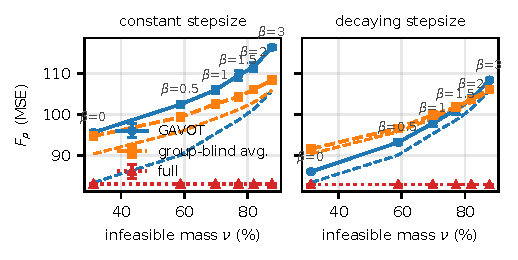
\includegraphics[width=\textwidth]{figs/severity_imdb.pdf}
\vspace{-14pt}
\caption{IMDb-Wiki severity sweep, measured $F_p$ (solid, $\pm1$ std)
against each rule's exact floor $\Phi$ (dashed). Left, constant stepsize,
where the residual swamps the alignment gain; right, decaying, where the
curves track their floors and transport wins until the floors close.}
\vspace{-8pt}
\label{fig:severity}
\end{figure*}

\begin{figure*}[t]
\centering

\includegraphics[width=\textwidth]{figs/rare_group_fit.pdf}
\vspace{-14pt}
\caption{Loss on the least represented groups, decaying stepsize, same runs
as Table~\ref{tab:overall}. Adult, cross-entropy on race Other
($p_i=0.2$); IMDb-Wiki, MSE on the $20$ top-importance identities, the
least observed once $\beta>0$.}
\vspace{-10pt}
\label{fig:rare}
\end{figure*}

Transport removes the bias of Proposition~\ref{prop:surrogate} but not the
variance, since a rare group receives a large weight when present. When
\eqref{eq:hall} fails no rule is unbiased for $\nabla F_p$, and Sinkhorn
scaling accumulates at a plan meeting $q$ whose row marginal
$\hat p\triangleq\Gamma\mathbf 1_J\in\Reach$ is the Kullback--Leibler
closest reachable point to $p$ \cite{csiszar1975,gietl2013ipfp,peyre2019};
%%CHECK direction of the KL and that [csiszar1975,gietl2013ipfp] give
%%      exactly this characterization of the limiting row marginal
Theorem~\ref{thm:rate} then holds with $\hat p$ for $p$, and groups with
$p_i>r_i$ are truncated at their observation rates. With
$\Phi(w)\triangleq F_p(\theta^\star_w)$, the target risk of the
$w$-optimal model (minimizers taken unique), any rule with effective
weighting $w$ satisfies
\begin{equation}
\E F_p(\bar\theta_T)-F_p(\theta^\star_p)
=\underbrace{\Phi(w)-\Phi(p)}_{\textnormal{\small alignment floor}}
+\underbrace{\E F_p(\bar\theta_T)-\Phi(w)}_{\textnormal{\small residual }\varepsilon_T(w)},
\label{eq:infeasible}
\end{equation}
with a floor that is nonnegative, at most $2M\|p-w\|_1$ and independent of
$T$, and a residual driven to zero by
$\E F_w(\bar\theta_T)-\min F_w\le DG/\sqrt{T}$. Transport ($w=\hat p$)
therefore beats uniform SGD or any other group-blind rule ($w=\tilde p$) at
horizon $T$ exactly when
\begin{equation}
\Delta_{\mathrm{floor}}\triangleq\Phi(\tilde p)-\Phi(\hat p)\;>\;
\varepsilon_T(\hat p)-\varepsilon_T(\tilde p).
\label{eq:gain}
\end{equation}
The \emph{alignment gain} on the left is fixed by the instance and
computable before training by solving two weighted problems; the right side
vanishes with $T$ but at finite $T$ depends on the stepsize and on the
variance of the rule, which transport inflates. No distance between
weightings decides the sign; \eqref{eq:gain} does.

% =====================================================================
\section{A Risk-Averse Reading of the Unreachable Part}
\label{sec:cvar}
% =====================================================================

Infeasible instances are common. When rare groups carry much of the target,
$\nu$ reaches $0.60$ on Adult and $0.88$ on IMDb-Wiki in Sec.~\ref{sec:exp},
$\hat p$ under-weights exactly the groups with $p_i>r_i$, their risks rise
by \eqref{eq:mono}, and since no rule leaves $\Reach$ the floor in
\eqref{eq:infeasible} cannot be removed by reweighting. What can change is
the question. Instead of one unreachable weighting, we ask for a guarantee
over all weightings the reachable one may stand for, which is the
distributionally robust reading of mean--CVaR
\cite{rockafellar2000cvar,rahimi2025agnostic,theodoropoulos2024restricted}.
For $w\in\simplex{N}$ and $\alpha,\gamma\in(0,1]$,
\begin{equation}
\begin{aligned}
F^{\alpha,\gamma}_w&\triangleq\gamma F_w+(1-\gamma)\,\CVaR^w_\alpha(f)
=\max\nolimits_{v\in\,\mathcal{U}_{\alpha,\gamma}(w)}F_v,\\
\mathcal{U}_{\alpha,\gamma}(w)&\triangleq\big\{v\in\simplex{N}:\
\gamma w\le v\le\kappa(\alpha,\gamma)\,w\big\},
\end{aligned}
\label{eq:meancvar}
\end{equation}
where $\CVaR^w_\alpha$ is taken over the group drawn from $w$; the equality
is the dual representation
$\CVaR^w_\alpha(f)=\max\{\sum_iu_if_i:u\in\simplex{N},\,u\le w/\alpha\}$
\cite{shapiro2009lectures} written in $v=\gamma w+(1-\gamma)u$.

For $\gamma<1$, Algorithm~\ref{alg:gavot} is projected stochastic
subgradient descent in $(\theta,\tau)\in\mathcal{C}\times[0,M]$ on the
jointly convex Rockafellar--Uryasev form
$\gamma F_{\hat p}(\theta)+(1-\gamma)\big(\tau+\frac1\alpha\sum_i\hat
p_i[f_i(\theta)-\tau]_+\big)$ of $F^{\alpha,\gamma}_{\hat p}$
\cite{rockafellar2000cvar}, whose subgradients are $\hat p$-weighted sums
of per-group terms (lines 5--7). Transport fixes \emph{which} weighting the
expectation is under, CVaR \emph{what} is averaged. The weights are at most
$\kappa(\alpha,\gamma)W$, so the argument of Theorem~\ref{thm:rate} gives
$\E F^{\alpha,\gamma}_{\hat p}(\bar\theta_T)-\min F^{\alpha,\gamma}_{\hat
p}=O(\kappa(\alpha,\gamma)/\sqrt{T})$ with exact group losses in the
indicators; the plug-in $\hat f^t_i$ adds a bias that vanishes with the
per-group sample size.
%%CHECK plug-in bias of 1{\hat f > tau}: exact if \hat f_i is computed on
%%      all of group i's data, as with 30-sample Adult groups?

The payoff is a certificate for the unreachable target. If
$p\in\mathcal{U}_{\alpha,\gamma}(\hat p)$, then $F_p\le
F^{\alpha,\gamma}_{\hat p}$ on $\mathcal{C}$ by \eqref{eq:meancvar}, so
\begin{equation}
\gamma\hat p\le p\le\kappa\hat p\ \Longrightarrow\
\E F_p(\bar\theta_T)\le\min_{\mathcal{C}}F^{\alpha,\gamma}_{\hat p}
+O\big(\kappa/\sqrt{T}\big).
\label{eq:certificate}
\end{equation}
Risk-neutral transport cannot see how far the truncated groups are
under-weighted, whereas the risk-averse layer places the whole target risk
under the quantity it drives down. With $\rho\triangleq\max_ip_i/\hat
p_i\ge1$, the premise of \eqref{eq:certificate} holds for
$\gamma\le\min_ip_i/\hat p_i$ and $\alpha\le(1-\gamma)/(\rho-\gamma)$, and
at $\gamma=0$, $\alpha\downarrow0$ the functional \eqref{eq:meancvar}
becomes the worst observed group. The price is a premium,
$\min F^{\alpha,\gamma}_{\hat p}\ge\min F_p$ since $p\in\mathcal{U}$, which
grows as $\alpha$ and $\gamma$ shrink.

% =====================================================================
\section{Experiments}
\label{sec:exp}
% =====================================================================
\hr{upsampling is not good because it removes stuff though what we want using everything data}
The analysis predicts that transport approaches full-access SGD where $p$ is
reachable, that elsewhere its advantage over group-blind weighting follows
\eqref{eq:gain} rather than the distance from $\hat p$ to $p$, and that the
rarest groups gain most. We test this on two tasks with severe imbalance,
sweeping availability from reachable to deeply unreachable. On Adult income
classification \cite{uci_adult}, logistic regression ($\eta{=}0.1$) is
trained on $100$ race-homogeneous groups of $30$ samples, with groups per
race proportional to prevalence ($85/10/3/1/1$) and a target uniform over
races, so the single group of a smallest race has $p_i=0.2$. On IMDb-Wiki
age regression \cite{rothe2018imdbwiki}, linear regression under
mean-squared error (MSE) on $128$-d face embeddings ($\eta{=}10^{-2}$)
covers $100$ identities with target $p_i\propto(101-i)^3$. Observation
rates follow $r\propto p^{\beta}$, $\beta\in\{0,\frac14,\frac12,\frac34,1\}$,
on Adult ($\nu$ from $0.60$ to $0$), and $r_i\propto i^{\beta}$,
$\beta\in\{0,\frac12,1,\frac32,2,3\}$, on IMDb-Wiki ($\nu$ from $0.31$ to
$0.88$), plus the aligned $r_i\propto 101-i$ ($\nu{=}0$). Each step the
sampler returns data from $K{=}3$ groups drawn $\propto r$, each
contributing the displacement of $H{=}5$ inner SGD steps from
$\theta^{t-1}$, combined by the rule's weights.
%%CHECK H=5 inner steps per group is what was run; the theory is for H=1
%%      (one weighted gradient per step). Either rerun with H=1 or keep
%%      this sentence. Also: "drawn prop. to r" vs r as the observation rate.
%%CHECK instance count: 5 Adult + 6 IMDb-Wiki + 1 aligned IMDb-Wiki = 12
Baselines are group-blind averaging, uniform over the observed groups
($\tilde p_i=r_i/K$), per-batch upsampling ($w_i\propto p_i/r_i$),
label-distribution smoothing (LDS) \cite{yang2021dir} for regression, the
fixed multiplier $(N/K)\,p_i$ \cite{rahimi2025fedavot}, and \emph{full},
which sees every group at every step weighted by $p$. All share
$\eta_t=\eta/(1+t/1000)$, fixed in advance; we run $4000$ steps over $5$
seeds, report $F_p$ over the last $500$, and compute each floor $\Phi$
exactly.

% ----------------------------------------------------------- Table 1
\begin{table}[t]
\centering
\caption{Headline $F_p$ (last $500$ steps, $5$ seeds). The fixed
multiplier gives $0.670$/$8504$ when infeasible, diverges when aligned.}
\label{tab:overall}
\small\setlength{\tabcolsep}{3pt}
\begin{tabular}{lccccc}
\toprule
Instance & \avot{} & blind avg. & upsamp. & LDS & full \\
\midrule
Adult, $\nu{=}0.60$ & $\best{0.2269}$ & $0.2479$ & $0.2288$ & -- & $0.2073$ \\
Adult, $\nu{=}0$   & $0.2075$ & $0.2077$ & $0.2075$ & -- & $0.2073$ \\
IMDb, $\nu{=}0.31$  & $\best{86.06}$ & $91.63$ & $86.74$ & $94.28$ & $82.95$ \\
IMDb, $\nu{=}0$    & $\best{84.28}$ & $86.37$ & $84.40$ & $89.43$ & $82.95$ \\
\bottomrule
\end{tabular}
\vspace{-8pt}
\end{table}

Transport wins three of the four headline cells (Table~\ref{tab:overall}),
$0.2269$ against $0.2479$ for group-blind averaging on Adult under
prevalence availability ($t{=}45$), and $86.06$ against $91.63$ ($t{=}21$)
and $84.28$ against $86.37$ ($t{=}13$) on IMDb-Wiki, closing $52\%$, $64\%$
and $61\%$ of the gap to full access without changing the sampler; on
aligned Adult both rules are within $4\cdot10^{-4}$ of full access, as
Proposition~\ref{prop:surrogate} predicts when $\tilde p\approx p$.
Upsampling recovers most of the gain and transport the rest ($t{=}5.8$ and
$2.6$ against it); LDS, which reweights by label rarity, trails even
group-blind averaging, and the unnormalized fixed multiplier is unstable.

The groups the target exists for gain most (Fig.~\ref{fig:rare}). On
Adult, transport lowers the cross-entropy of race Other at every skew,
$0.073$ against $0.119$ under prevalence availability (full $0.031$). On
IMDb-Wiki the top-importance identities improve at every $\nu\le0.70$
($77.0$ against $86.4$ at $\nu{=}0.31$, full $72.2$, and $253$ against
$331$ on the most starved identity) and lose at the three most infeasible
skews, one step before $F_p$ does.

% ----------------------------------------------------------- Table 2
\begin{table}[t]
\centering
\caption{IMDb-Wiki sweep, decaying stepsize; Welch $t$ of the gain.}
\label{tab:severity}
\small\setlength{\tabcolsep}{4.2pt}
\begin{tabular}{lcccccc}
\toprule
$\beta$ & $0$ & $0.5$ & $1.0$ & $1.5$ & $2.0$ & $3.0$ \\
$\nu$ & $0.31$ & $0.59$ & $0.70$ & $0.77$ & $0.82$ & $0.88$ \\
\midrule
$\Delta_{\mathrm{floor}}$ & $6.99$ & $5.71$ & $3.67$ & $2.56$ & $1.62$ & $0.02$ \\
gain & $\best{+5.57}$ & $\best{+3.46}$ & $\best{+2.05}$ & $+0.58$ & $-0.03$ & $-2.28$ \\
$t$ & $20.7$ & $11.3$ & $5.4$ & $1.1$ & $-0.1$ & $-7.9$ \\
\bottomrule
\end{tabular}
\vspace{-8pt}
\end{table}

The sharpest prediction concerns that crossover. As $\nu$ grows on
IMDb-Wiki, $\hat p$ and $\tilde p$ truncate the same groups and
$\Delta_{\mathrm{floor}}$ falls from $6.99$ to $0.02$
(Table~\ref{tab:severity}). The measured gain sits below
$\Delta_{\mathrm{floor}}$ by a nearly constant residual, mean $1.9$, and
its sign flips where $\Delta_{\mathrm{floor}}$ crosses that value, between
$\beta=1.5$ and $2$, as \eqref{eq:gain} predicts, whereas
$\|p-\hat p\|_1<\|p-\tilde p\|_1$ holds in every instance, losses
included. On Adult (not tabulated) the gain tracks or exceeds
$\Delta_{\mathrm{floor}}$ at every skew. Before the first gradient step, a large gain thus predicts a
win and a vanishing one a contest decided by variance.

Variance is where the stepsize enters. At constant stepsize
(Fig.~\ref{fig:severity}, left) transport loses on all six IMDb-Wiki skews,
by up to $7.9$,
%%CHECK "by up to 7.9": MSE or the Welch t? (Table 2 has t = -7.9 at beta=3)
since the large weight it puts on a starved group raises the noise floor on
which constant-step iterates settle. Under the decaying schedule that floor
vanishes, the curves meet their dashed floors, and only the residual
remains, $2.3$ at $\nu{=}0.88$, the one significant loss.

Finally, the premium of the risk-averse layer is real. On a $10\times10$
$(\alpha,\gamma)$ grid, $F_p$ is minimized on the $\gamma=1$ edge in every
instance. The layer helps the worst race of Adult under prevalence
availability, $0.3624$ at $(\alpha,\gamma)=(0.2,0.7)$ against $0.3679$ for
\avot{} and $0.3994$ group-blind, but never the least represented group,
whose best grid loss is at $\gamma=1$ in all headline instances, since CVaR
reweights only the groups present in a batch and multiplies weights already
of order $p_i/r_i$; it is a guarantee, not a way to lower the average.

% =====================================================================
\vspace{-4pt}
\section{Conclusion}
% =====================================================================

SGD fails group fairness at the batch weights, which follow the sampler,
not the declared importance. Masked transport reaches every reachable
target at the rate of full-access SGD; otherwise a gain computable before
training predicts whether it pays, and mean--CVaR certifies the rest.
The nonconvex case remains open.

% =====================================================================
\clearpage
\renewcommand{\refname}{REFERENCES}

\balance
\begin{thebibliography}{99}\setlength{\itemsep}{-2pt}\small

\bibitem{buolamwini2018gender}
J.~Buolamwini and T.~Gebru, ``Gender shades: Intersectional accuracy disparities
in commercial gender classification,'' in \emph{Proc. FAT*}, 2018, pp. 77--91.

\bibitem{koenecke2020speech}
A.~Koenecke, A.~Nam, E.~Lake, J.~Nudell, M.~Quartey, Z.~Mengesha, C.~Toups,
J.~R. Rickford, D.~Jurafsky, and S.~Goel, ``Racial disparities in automated
speech recognition,'' \emph{Proc. Natl. Acad. Sci. USA}, vol.~117, no.~14,
pp. 7684--7689, 2020.

\bibitem{yang2021dir}
Y.~Yang, K.~Zha, Y.-C. Chen, H.~Wang, and D.~Katabi, ``Delving into deep
imbalanced regression,'' in \emph{Proc. ICML},
2021, pp. 11842--11851.

\bibitem{hashimoto2018repeated}
T.~Hashimoto, M.~Srivastava, H.~Namkoong, and P.~Liang, ``Fairness without
demographics in repeated loss minimization,'' in \emph{Proc. ICML}, 2018, pp. 1929--1938.

\bibitem{he2009imbalanced}
H.~He and E.~A. Garcia, ``Learning from imbalanced data,'' \emph{IEEE Trans.
Knowl. Data Eng.}, vol.~21, no.~9, pp. 1263--1284, 2009.

\bibitem{mohri2019agnostic}
M.~Mohri, G.~Sivek, and A.~T. Suresh, ``Agnostic federated learning,'' in
\emph{Proc. ICML}, 2019, pp. 4615--4625.

\bibitem{li2020fair}
T.~Li, M.~Sanjabi, A.~Beirami, and V.~Smith, ``Fair resource allocation in
federated learning,'' in \emph{Proc. ICLR}, 2020.

\bibitem{chawla2002smote}
N.~V. Chawla, K.~W. Bowyer, L.~O. Hall, and W.~P. Kegelmeyer, ``SMOTE:
Synthetic minority over-sampling technique,'' \emph{J. Artif. Intell. Res.},
vol.~16, pp. 321--357, 2002.

\bibitem{idrissi2022simple}
B.~Y. Idrissi, M.~Arjovsky, M.~Pezeshki, and D.~Lopez-Paz, ``Simple data
balancing achieves competitive worst-group-accuracy,'' in \emph{Proc. CLeaR}, 2022, pp. 336--351.

\bibitem{cui2019classbalanced}
Y.~Cui, M.~Jia, T.-Y. Lin, Y.~Song, and S.~Belongie, ``Class-balanced loss
based on effective number of samples,'' in \emph{Proc. IEEE/CVF CVPR}, 2019, pp. 9268--9277.

\bibitem{cao2019ldam}
K.~Cao, C.~Wei, A.~Gaidon, N.~Arechiga, and T.~Ma, ``Learning imbalanced
datasets with label-distribution-aware margin loss,'' in \emph{Proc. NeurIPS}, vol.~32, 2019.

\bibitem{menon2021logit}
A.~K. Menon, S.~Jayasumana, A.~S. Rawat, H.~Jain, A.~Veit, and S.~Kumar,
``Long-tail learning via logit adjustment,'' in \emph{Proc. ICLR}, 2021.

\bibitem{byrd2019importance}
J.~Byrd and Z.~C. Lipton, ``What is the effect of importance weighting in deep
learning?'' in \emph{Proc. ICML}, 2019, pp.
872--881.

\bibitem{needell2014sgd}
D.~Needell, R.~Ward, and N.~Srebro, ``Stochastic gradient descent, weighted
sampling, and the randomized Kaczmarz algorithm,'' in \emph{Proc. NeurIPS}, vol.~27, 2014, pp. 1017--1025.

\bibitem{katharopoulos2018not}
A.~Katharopoulos and F.~Fleuret, ``Not all samples are created equal: Deep
learning with importance sampling,'' in \emph{Proc. ICML}, 2018, pp. 2525--2534.

\bibitem{sagawa2020dro}
S.~Sagawa, P.~W. Koh, T.~Hashimoto, and P.~Liang, ``Distributionally robust
neural networks for group shifts,'' in \emph{Proc. ICLR}, 2020.

\bibitem{liu2021jtt}
E.~Z. Liu, B.~Haghgoo, A.~S. Chen, A.~Raghunathan, P.~W. Koh, S.~Sagawa,
P.~Liang, and C.~Finn, ``Just train twice: Improving group robustness without
training group information,'' in \emph{Proc. ICML}, 2021, pp. 6781--6792.

\bibitem{namkoong2017variance}
H.~Namkoong and J.~C. Duchi, ``Variance-based regularization with convex
objectives,'' in \emph{Proc. NeurIPS}, vol.~30,
2017, pp. 2971--2980.

\bibitem{levy2020large}
D.~Levy, Y.~Carmon, J.~C. Duchi, and A.~Sidford, ``Large-scale methods for
distributionally robust optimization,'' in \emph{Proc. NeurIPS}, vol.~33, 2020, pp. 8847--8860.

\bibitem{curi2020adaptive}
S.~Curi, K.~Y. Levy, S.~Jegelka, and A.~Krause, ``Adaptive sampling for
stochastic risk-averse learning,'' in \emph{Proc. NeurIPS}, vol.~33, 2020, pp. 1036--1047.

\bibitem{hardt2016equality}
M.~Hardt, E.~Price, and N.~Srebro, ``Equality of opportunity in supervised
learning,'' in \emph{Proc. NeurIPS}, vol.~29,
2016, pp. 3315--3323.

\bibitem{agarwal2018reductions}
A.~Agarwal, A.~Beygelzimer, M.~Dud\'{i}k, J.~Langford, and H.~Wallach, ``A
reductions approach to fair classification,'' in \emph{Proc. ICML}, 2018, pp. 60--69.

\bibitem{cotter2019twoplayer}
A.~Cotter, H.~Jiang, and K.~Sridharan, ``Two-player games for efficient
non-convex constrained optimization,'' in \emph{Proc. ALT}, 2019, pp. 300--332.

\bibitem{chamon2020pacc}
L.~F.~O. Chamon and A.~Ribeiro, ``Probably approximately correct constrained
learning,'' in \emph{Proc. NeurIPS}, vol.~33, 2020,
pp. 16722--16735.

\bibitem{chamon2023nonconvex}
L.~F.~O. Chamon, S.~Paternain, M.~Calvo-Fullana, and A.~Ribeiro, ``Constrained
learning with non-convex losses,'' \emph{IEEE Trans. Inf. Theory}, vol.~69,
no.~3, pp. 1739--1760, 2023.

\bibitem{rahimi2025fedavot}
H.~Rahimi and D.~Kalogerias, ``FedAVOT: Exact distribution alignment in
federated learning via masked optimal transport,'' in \emph{Proc. IEEE ICASSP}, 2026.

\bibitem{rahimi2026federage}
H.~Rahimi and D.~Kalogerias, ``FedeRage: Provably convergent agnostic
federated learning under general client drift,'' arXiv:2609.21057, 2026.
% reference supplied by Herlock on Discord, 2026-09-21 (replaces the exact-penalty placeholder)

\bibitem{rahimi2025agnostic}
H.~Rahimi and D.~Kalogerias, ``Convergence of agnostic federated averaging,''
in \emph{Proc. IEEE CAMSAP}, 2025.

\bibitem{villani2009}
C.~Villani, \emph{Optimal Transport: Old and New}. Springer, 2009.

\bibitem{peyre2019}
G.~Peyr\'{e} and M.~Cuturi, \emph{Computational Optimal Transport}. Now
Publishers, 2019.

\bibitem{hall1935}
P.~Hall, ``On representatives of subsets,'' \emph{J. London Math. Soc.},
vol.~10, no.~1, pp. 26--30, 1935.

\bibitem{fordfulkerson1956}
L.~R. Ford and D.~R. Fulkerson, ``Maximal flow through a network,'' \emph{Canad.
J. Math.}, vol.~8, pp. 399--404, 1956.

\bibitem{sinkhorn1967}
R.~Sinkhorn, ``Diagonal equivalence to matrices with prescribed row and column
sums,'' \emph{Amer. Math. Monthly}, vol.~74, no.~4, pp. 402--405, 1967.

\bibitem{cuturi2013}
M.~Cuturi, ``Sinkhorn distances: Lightspeed computation of optimal transport,''
in \emph{Proc. NeurIPS}, vol.~26, 2013, pp.
2292--2300.

\bibitem{nemirovski2009}
A.~Nemirovski, A.~Juditsky, G.~Lan, and A.~Shapiro, ``Robust stochastic
approximation approach to stochastic programming,'' \emph{SIAM J. Optim.},
vol.~19, no.~4, pp. 1574--1609, 2009.

\bibitem{csiszar1975}
I.~Csisz\'{a}r, ``$I$-divergence geometry of probability distributions and
minimization problems,'' \emph{Ann. Probab.}, vol.~3, no.~1, pp. 146--158, 1975.

\bibitem{gietl2013ipfp}
C.~Gietl and F.~P. Reffel, ``Accumulation points of the iterative proportional
fitting procedure,'' \emph{Statistics}, vol.~47, no.~6, pp. 1321--1335, 2013.

\bibitem{rockafellar2000cvar}
R.~T. Rockafellar and S.~Uryasev, ``Optimization of conditional value-at-risk,''
\emph{J. Risk}, vol.~2, no.~3, pp. 21--41, 2000.

\bibitem{theodoropoulos2024restricted}
P.~Theodoropoulos, K.~E. Nikolakakis, and D.~Kalogerias, ``Federated learning
under restricted user availability,'' in \emph{Proc. IEEE ICASSP}, 2024.

\bibitem{shapiro2009lectures}
A.~Shapiro, D.~Dentcheva, and A.~Ruszczy\'{n}ski, \emph{Lectures on
Stochastic Programming: Modeling and Theory}. SIAM, 2009.

\bibitem{uci_adult}
B.~Becker and R.~Kohavi, ``Adult,'' UCI Machine Learning Repository, 1996.
[Online]. Available: https://doi.org/10.24432/C5XW20

\bibitem{rothe2018imdbwiki}
R.~Rothe, R.~Timofte, and L.~Van~Gool, ``Deep expectation of real and apparent
age from a single image without facial landmarks,'' \emph{Int. J. Comput.
Vis.}, vol.~126, no.~2--4, pp. 144--157, 2018.

\end{thebibliography}

\end{document}